\begin{comment}


% \begin{figure}
%   \makebox[\textwidth][c]{
%   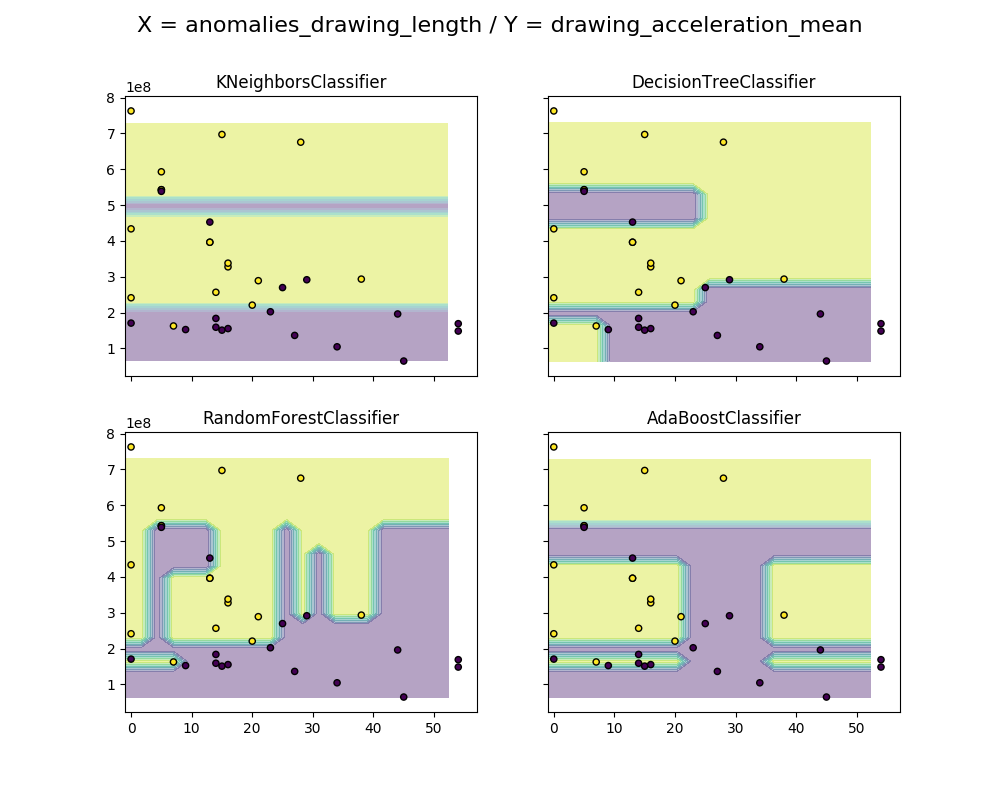
\includegraphics[width=1.7\textwidth]{images/classifier/001}}%
%   \caption{Caption}
%   \label{fig:key}
% \end{figure}


% Our aim was to build a discriminative model to differentiate between people with PD and HC. It is a binary classification task that can be resolved by statistical machine learning algorithms.

% The underlying idea of SVM classifiers is to calculate a maximal margin hyperplane separating two classes of the data. To learn non-linearly separable functions, the data are implicitly mapped to a higher dimensional space by means of a kernel function, where a separating hyperplane is found. New samples are classified according to the side of the hyperplane they belong to. 

% Decision Trees (DTs) are a non-parametric supervised learning method used for classification and regression. Decision trees learn from data to approximate a sine curve with a set of if-then-else decision rules. The deeper the tree, the more complex the decision rules and the fitter the model.

% Decision tree builds classification or regression models in the form of a tree structure. It breaks down a data set into smaller and smaller subsets while at the same time an associated decision tree is incrementally developed. The final result is a tree with decision nodes and leaf nodes. A decision node has two or more branches. Leaf node represents a classification or decision. The topmost decision node in a tree which corresponds to the best predictor called root node. Decision trees can handle both categorical and numerical data.

% each capable of producing a response when presented with a set of predictor values. For classification problems, this response takes the form of a class membership classifies, a set of independent predictor values with one of the categories present in the dependent variable.

% The essence of the technique is to construct multiple decision trees in randomly selected feature sub-space and use averaging to improve the predictive accuracy and control over-fitting. Using tree ensembles can lead to significant improvement in prediction accuracy (i.e., better ability to predict new data cases).

% Random forests or random decision forests are an ensemble learning method for classification, regression and other tasks, that operate by constructing a multitude of decision trees at training time and outputting the class that is the mode of the classes (classification) or mean prediction (regression) of the individual trees

% AdaBoost, short for Adaptive Boosting, is a machine learning meta-algorithm formulated by Yoav Freund and Robert Schapire, who won the 2003 Gödel Prize for their work. It can be used in conjunction with many other types of learning algorithms to improve performance. The output of the other learning algorithms ('weak learners') is combined into a weighted sum that represents the final output of the boosted classifier. AdaBoost is adaptive in the sense that subsequent weak learners are tweaked in favor of those instances misclassified by previous classifiers. AdaBoost is sensitive to noisy data and outliers. In some problems it can be less susceptible to the overfitting problem than other learning algorithms. The individual learners can be weak, but as long as the performance of each one is slightly better than random guessing, the final model can be proven to converge to a strong learner.

% AdaBoost is one of the important ensemble methods known as boosting. The key idea behind boosting techniques is to use ensemble methods to combine weak classifiers in order to build a strong learner. AdaBoost is an iterative boosting algorithm constructing a strong classifier as a linear combination of weak classifiers, each performing at least above chance level (50 correct classification). 

% We used decision trees classifiers as weak classifiers. The maximum number of estimators at which boosting is terminated was set to 500. Settings used for decision trees were as follows. The number of features to consider when looking for the best split was the square root of the number of features and the maximum depth of the tree was set to 3.

% Classifier validation was conducted using stratified 10-fold cross-validation. The data was divided into ten mutually exclusive and exhaustive equal-sized subsets. For each subset, the union of all other subsets was considered as training data and the error rate was determined. Errors over different subsets were averaged to obtain the classification error. The process was repeated a total of ten times; the original dataset was randomly permuted in each repetition prior to splitting into training and testing subsets. The results were averaged over all ten runs.
% The classification test performance was determined by the classification accuracy Pacc, sensitivity Psen and specificity Pspe.

% From all computed features we kept only those that passed the Mann–Whitney U test, i.e. those that showed a statistically significant (p < 0.05) difference between the PD and control groups. Table 3 shows 20 most relevant features and median of their values for PD and healthy control group. Features are sorted according Spearman’s correlation coefficient 
% The highest classification accuracy using pressure features Pacc = 74.2\% was obtained for data from the task 6

to apply 3-fold cross-validation, more specific This cross-validation object is a variation of KFold that returns stratified folds. The folds are made by preserving the percentage of samples for each class.

Stratified K-Folds cross-validator

Provides train/test indices to split data in train/test sets.
This cross-validation object is a variation of KFold that returns stratified folds. The folds are made by preserving the percentage of samples for each class.

StratifiedKFold implementation of $Scikit-learn$

% Classifier validation was conducted using stratified 10-fold cross-validation. The data was divided into ten mutually exclusive and exhaustive equal-sized subsets. For each subset, the union of all other subsets was considered as training data and the error rate was determined. Errors over different subsets were averaged to obtain the classification error. The process was repeated a total of ten times; the original dataset was randomly permuted in each repetition prior to splitting into training and testing subsets. The results were averaged over all ten runs.

% The classification test performance was determined by the classification accuracy Pacc, sensitivity Psen and specificity Pspe.
% From all computed features we kept only those that passed the Mann–Whitney U test, i.e. those that showed a statistically significant (p < 0.05) difference between the PD and control groups. Table 3 shows 20 most relevant features and median of their val- ues for PD and healthy control group. Features are sorted according Spearman’s correlation coefficient.

% % % % % % % % % % % % % % % % % % % % % % % % % % % % % % % % % % % %

% One round of cross-validation involves partitioning a sample of data into complementary subsets, performing the analysis on one subset (called the training set), and validating the analysis on the other subset (called the validation set or testing set). To reduce variability, in most methods multiple rounds of cross-validation are performed using different partitions, and the validation results are combined (e.g. averaged) over the rounds to estimate a final predictive model.

% One of the main reasons for using cross-validation instead of using the conventional validation (e.g. partitioning the data set into two sets of 70\% for training and 30% for test) is that there is not enough data available to partition it into separate training and test sets without losing significant modelling or testing capability. In these cases, a fair way to properly estimate model prediction performance is to use cross-validation as a powerful general technique.[5]



\end{comment}

As demonstrated in a recent research by Farzan Majeed Noori,
Benedikte Wallace, Md. Zia Uddin and Jim Torresen in \cite{10.1007/978-3-030-20205-7_25}, a combined architecture of using OpenPose for pose estimation and Recurrent Neural Networks (RNN) for human activity recognition could prove as the new state-of-the-art solution for robust and non-intrusive human activity recognition. In the cited research, OpenPose was used to extract keypoints from a subset of the Berkeley Multimodal Human Action Database (BMHAD) \cite{Berkeley-MHAD}. What makes it remarkable, is the classification accuracy obtained using a Recurrent Neural Network with Long Short-term Memory (LSTM) cells over more conventional machine learning classifiers, such as Support Vector Machines, Decision Trees and Random Forests. Since the dataset contained human activities recorded from different angles, the solution is also view-invariant, which also increases the robustness of this solution. Another paper, a technical report by Chinmay Sawant \cite{sawant2020human}, also supports the combination of OpenPose with LSTMs for time-series classification, reporting similar accuracy results in real-time application on the same BMHAD dataset, making use of the efficiency of this solution.

The difference of the cited work and current work is the custom dataset constructed for gymnastics based movements. In contrast to the BMHAD dataset, which includes 11 general activities, such as jumping jacks, waving and clapping, the dataset used in the current thesis uses more complex biomechanical activities, including human body rotations and airtime, such as backflips and back-handsprings. The author of this paper expects RNNs used for general action recognition to also be applicable to gymnastics movements. The goal of this research is to validate this hypothesis and investigate neural networks most suitable for gymnastics action recognition. 

\section{Methodology}

To develop neural networks capable of recognizing gymnastics movements, a combination of empirical knowledge with the mathematical theory of artificial neural networks is used as the starting point. The development process starts by training a simple recurrent neural network with gymnastics data and analyzing the results. Simple RNN is chosen primarily for its known property of being able to represent information from context window \cite{DBLP:journals/corr/Lipton15}. RNNs have \textit{long-term memory} in the form of weights, enabling the network to \textit{remember} a gymnastics element represented as a sequence. An iterative process is used to train, validate, analyze and compare the results of each classifier. The steps followed in the current thesis are represented in figure \ref{classifier-tasks}.

\begin{figure}[htb]
  \centering
    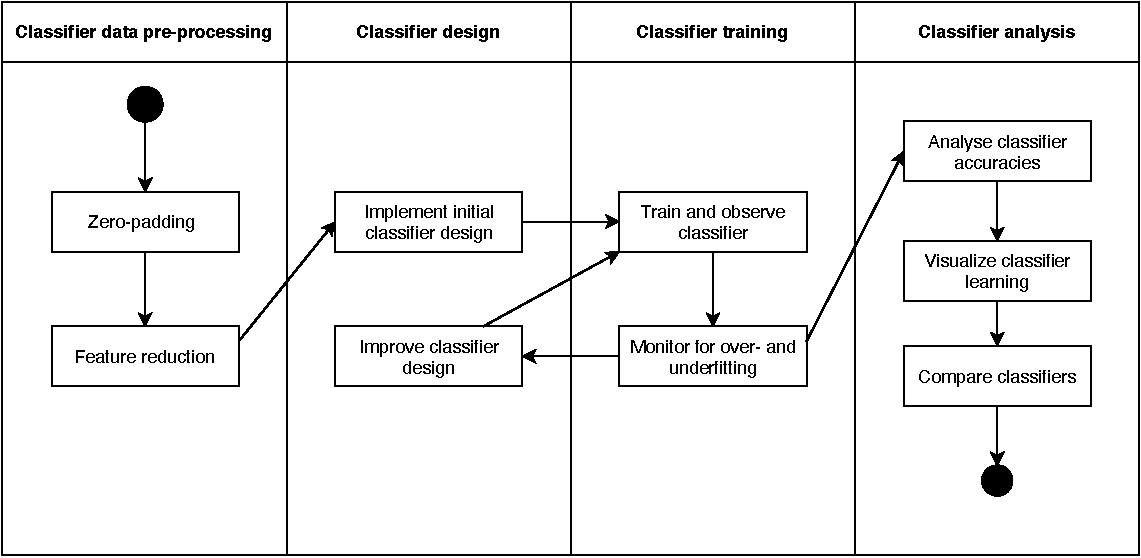
\includegraphics[width=\textwidth,keepaspectratio]
    {images/classifier/classifier-tasks}
    \caption{Tasks completed regarding classifier development in the thesis}
    \label{classifier-tasks}
\end{figure}

\subsection{Classifier Prerequisites}

Two prerequisites before feeding training data to the classifiers include:

\begin{easylist}[itemize]

& \textit{Zero-padding} --- Gymnastics activities performed vary in their length and in order to keep the classifier dimensions static, the samples are zero-padded. Zero-padding is done by finding the longest sample performed and increasing the timesteps of other samples with zero values until they are equal in length to the longest sample. 
& \textit{Feature reduction} --- Recurrent neural networks are prone to overfitting and with the combination of the author's domain knowledge about gymnastics, the 25 total keypoints obtained during pose estimation are reduced to 15, filtering out less prominent keypoints necessary to recognize gymnastics movements. The 15 keypoints used for classification include the trunk, head and limbs of the skeleton.

\end{easylist}


\subsection{Classifier Algorithms}

Classifier algorithms experimented with in the thesis are:

\begin{easylist}[itemize]

& \textit{Simple RNN} --- The first classifier (shown in figure \ref{simple-rnn-network-layers}) experimented with is a network model with one simple recurrent layer. The recurrent layer consists of 2 units, chosen accordingly to the amount of outputs the network produces - the movements is either a backflip or a back handspring. A dropout layer with a 0.5 rate to prevent overfitting is added next. An activation layer with rectified linear units follows with a flattening layer to reduce dimensions and finally an output layer with softmax activation is used for representing the different activities. Categorical cross entropy is used as the loss function during stochastic gradient descent with an Adam optimizer with a learning rate of 0.001. 
& \textit{Hierarchical RNN} --- The Simple RNN works well for the short duration activities analyzed in this paper, but the downside of using one recurrent layer is observability. By feeding all available dimensions into one recurrent layer, we lose the visibility of what exactly the different units in a neural network learn. A more advanced and deeper neural network (inspired by article \cite{hierarchical-rnn-har}) consists of several recurrent layers, each representing some logical unit. The model used for experimentation in this paper is shown in figure \ref{hierarchical-rnn-network-layers}. Hierarchical RNN uses multiple input units, each representing a human skeleton subsection. In this example, the skeleton is divided into left arm, right arm, trunk, left leg and right leg subsections. In subsequent layers, the recurrent units are fused together and finally neural activations are applied on a fully connected skeleton layer. One of the advantages of this method is that we can now intercept some layer of interest and observe the neuron activations only regarding a subsection of the skeleton.
& \textit{LSTM} --- An RNN with LSTM cells was also implemented. The simple recurrent layer is substituted with a hidden LSTM layer with 2 hidden units accordingly representing the outputs of the network. Other layers remain identical with the \textit{Simple RNN} classifier.

\end{easylist}

\begin{figure}[htb]
  \centering
    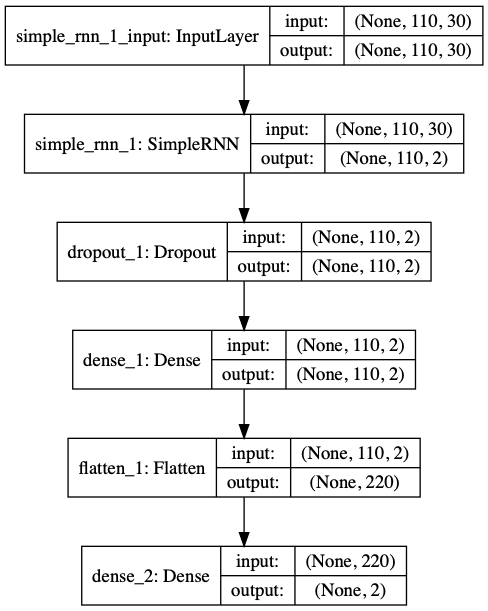
\includegraphics[width=0.7\textwidth,keepaspectratio]
    {images/classifier/simple-rnn-network-layers}
    \caption{The neural network design with a simple recurrent layer}
    \label{simple-rnn-network-layers}
\end{figure}

\begin{figure}[htb]
  \centering
    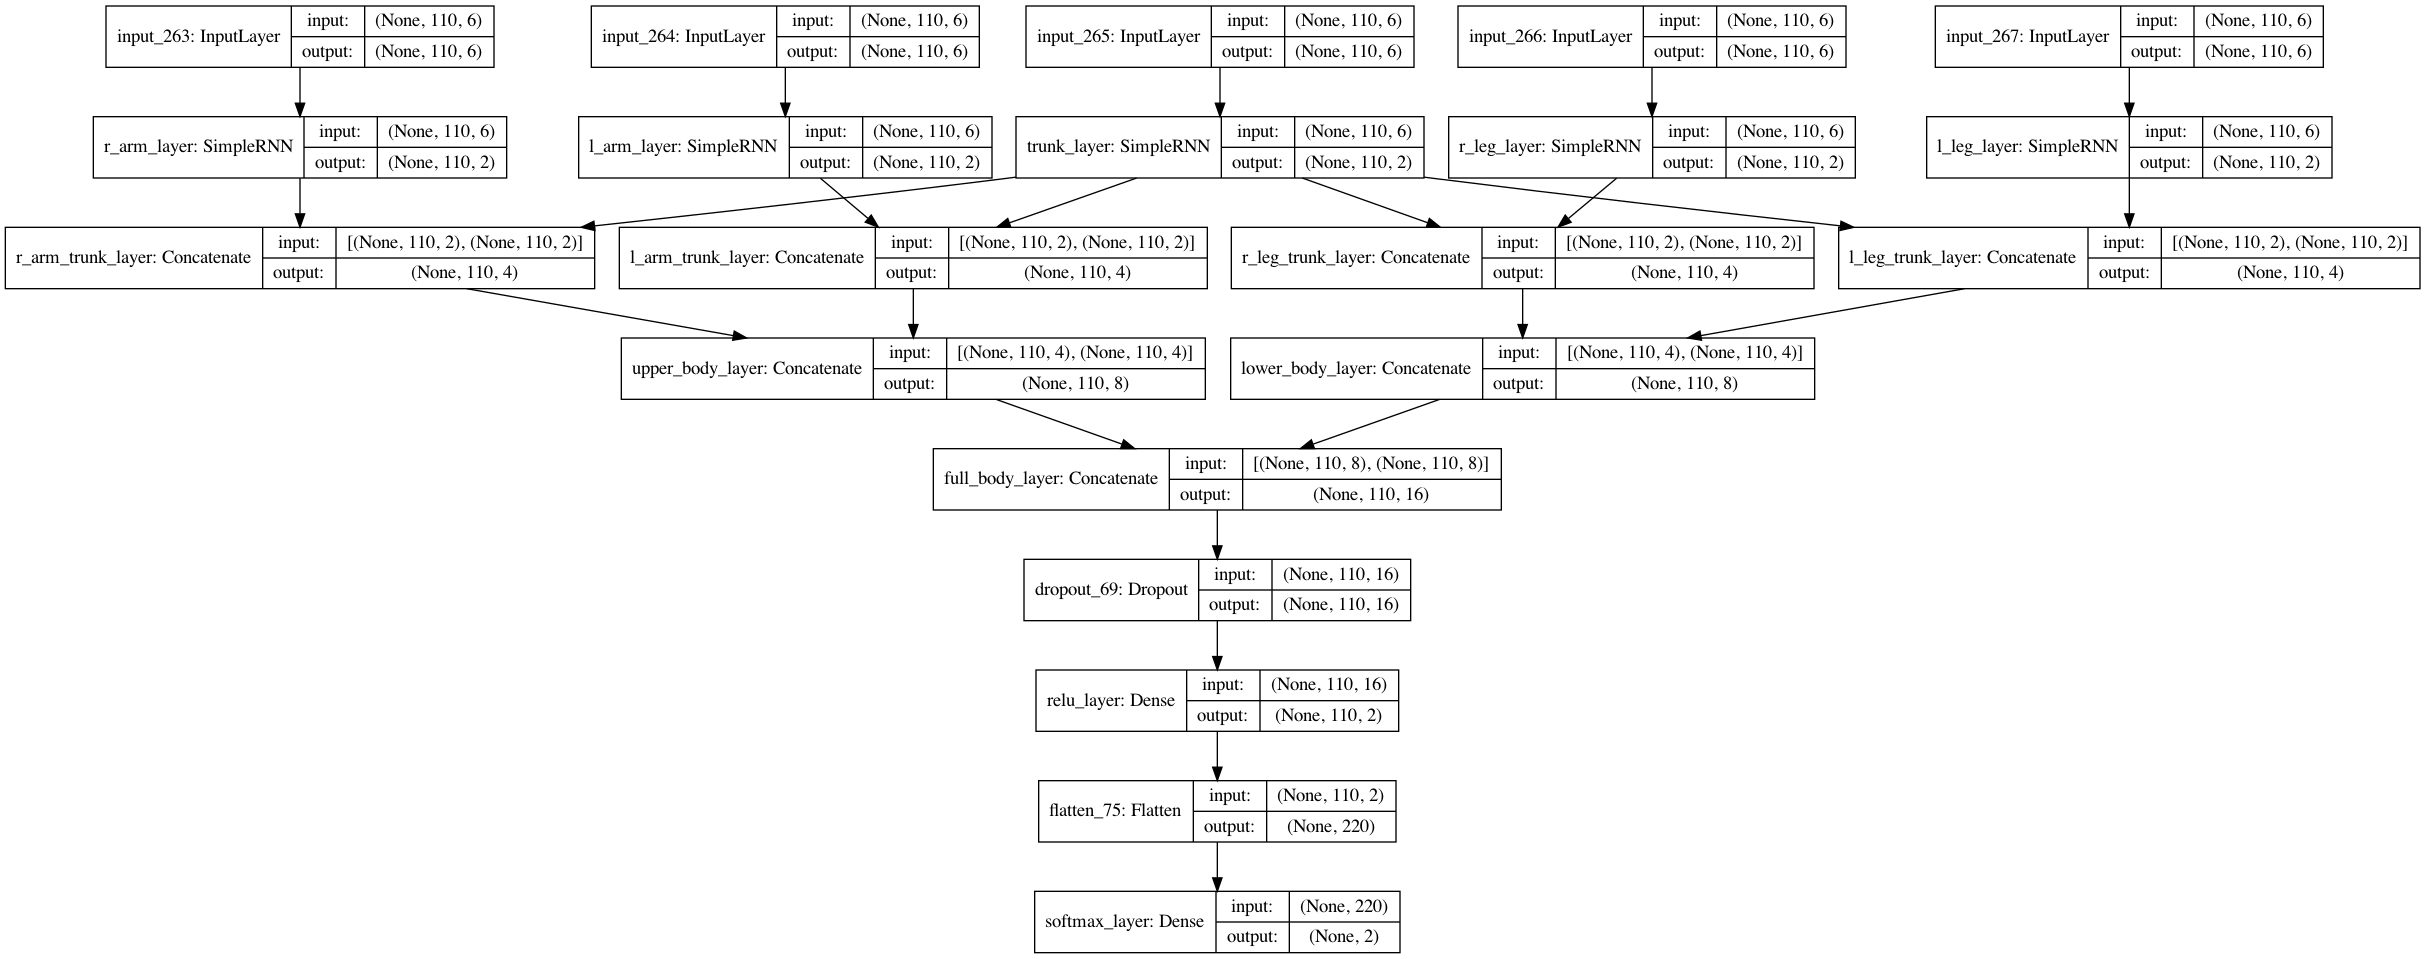
\includegraphics[width=\textwidth,keepaspectratio]
    {images/classifier/hierarchical-rnn-model-summary}
    \caption{The neural network design with hierarchical recurrent layers}
    \label{hierarchical-rnn-network-layers}
\end{figure}

\subsection{Classifier Validation}

Validating the correctness of our RNN training requires the usage of some common classifier validation techniques. These techniques are commonly used while training neural networks to avoid overfitting. 

Firstly, the sample data is split by 0.2 rate between training and testing data in order to test for unbiased results when the model training has stopped. A validation split of 0.33 rate is also used while training the RNN to observe the loss and accuracy of the model, essential to help with hyperparameter tuning. Validation set is kept separately from test set so when we optimize our hyperparameters, we can validate our results against the test set. The figure \ref{model-validation-monitoring} demonstrates how the LSTM model accuracy and loss are monitored during epochs in order to detect overfitting or underfitting. When the training and test set accuracies and losses do not diverge too much, we can be more confident that our classifier is generalizing and not just optimizing for the input data \cite{deep-learning-cookbook}.

Lastly, the experiment is repeated on 5 unconnected models. Neural networks sometimes tend to converge to some minima that is not the most optimal (global). By running our experiment on 5 unconnected models, we avoid basing our observations and analysis under the influence of one sub-optimal (local) minima. 

\begin{figure*}
   \centering
\begin{tabular}{cc}
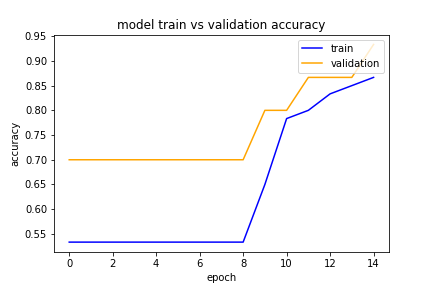
\includegraphics[width=7.5cm]{images/classifier/model-train-vs-validation-accuracy}&
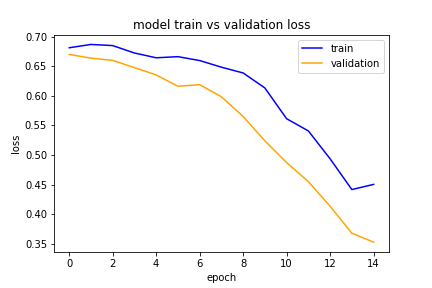
\includegraphics[width=7.5cm]{images/classifier/model-train-vs-validation-loss}\\
\end{tabular}
    \caption{Monitoring for model accuracy and loss to detect overfitting/underfitting}
    \label{model-validation-monitoring}
\end{figure*}

\subsection{Classifier Training Process}

\subsubsection{Simple RNN} 

Due to the small sample data size, the RNN classifier is trained for 5 epochs with stochastic gradient descent. The hyperparameters are empirically selected for the classifier, with the goal to maximize the accuracy while preventing overfitting.

An early stopping hook is also implemented to monitor for validation loss improvements. No improvements in validation loss commonly indicate that the network has stopped learning and is starting to overfit to the training data. After 3 epochs with no improvements the hook stops the learning process of the neural network. 

\begin{figure*}
    \centering
\begin{tabular}{c|c}
    \bfseries Repeat & \bfseries Accuracy (\%) % specify table head
    \csvreader[head to column names]{simple-rnn-repeats-accuracy.csv}{} % use head of csv as column names
    {\\\hline\i & \a} % specify your coloumns here
\end{tabular}
    \caption{Mean accuracies obtained during each Simple RNN classifier run}
    \label{simple-rnn-repeats-accuracy}
\end{figure*}

\section{Classifier Visualization and Analysis}

\subsubsection{Simple RNN} 

The fourth experiment run (from table \ref{simple-rnn-repeats-accuracy}) is chosen to dive deeper into the inner workings of the classifier.

By configuring the model's RNN layer to return hidden states, it is possible to intercept the output values of this layer and investigate the neuron activations. It is also possible to visualize these activations to better understand what the neurons are learning. The author compares neuron activations of backflips (figure \ref{backflip-neuron-activations-simple-rnn}) and back handsprings (figure \ref{back-handspring-neuron-activations-simple-rnn}). In both figures, the activations are visualized using four horizontal lines. Each horizontal line also consists of three inner lines, where the first represents timestep indices and other two represent activations of two hidden layer neurons. The outer horizontal lines are split by 30 timesteps, which correspond to 0.5 seconds of activity time since the activities are recorded at 60 frames per second.

All samples are 110 timesteps long and the missing values are zero-padded. The chosen samples are also correctly predicted by the model. It is interesting to observe how the first neuron starts to flicker it's activation when it encounters the ending of an activity. From here we can also observe how back handsprings tend to last longer than backflips, easily noticeable from neuron activations. A second observation can be made by noticing that the first neuron seems to activate throughout almost the whole duration of a backflip. 

TODO: Add reference to visualization source

\begin{figure*}
   \centering
\begin{tabular}{c}
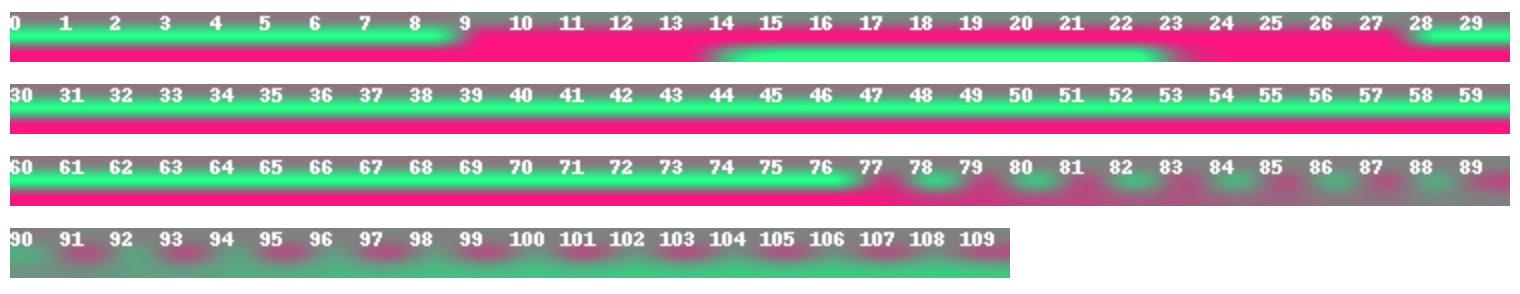
\includegraphics[width=\textwidth]{images/classifier/neuron-activations-simple-rnn-model-3/backflip-23-tiit}\\
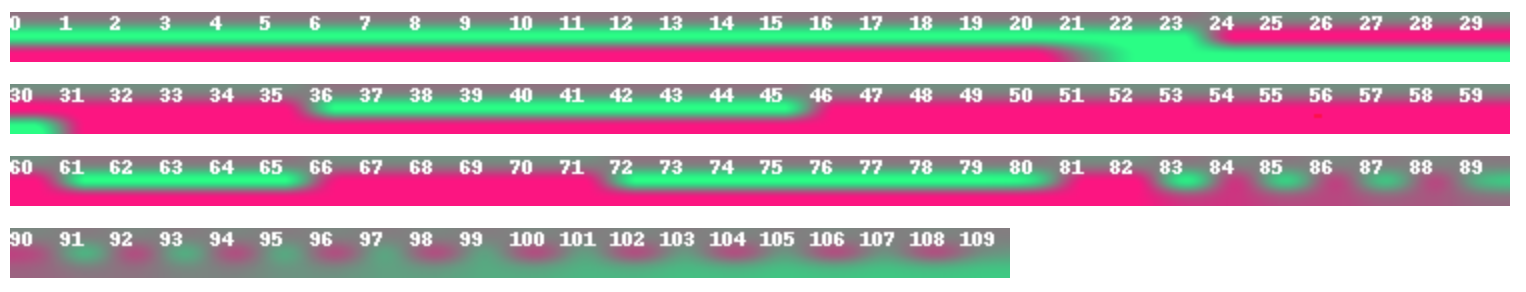
\includegraphics[width=\textwidth]{images/classifier/neuron-activations-simple-rnn-model-3/backflip-40-margus}\\
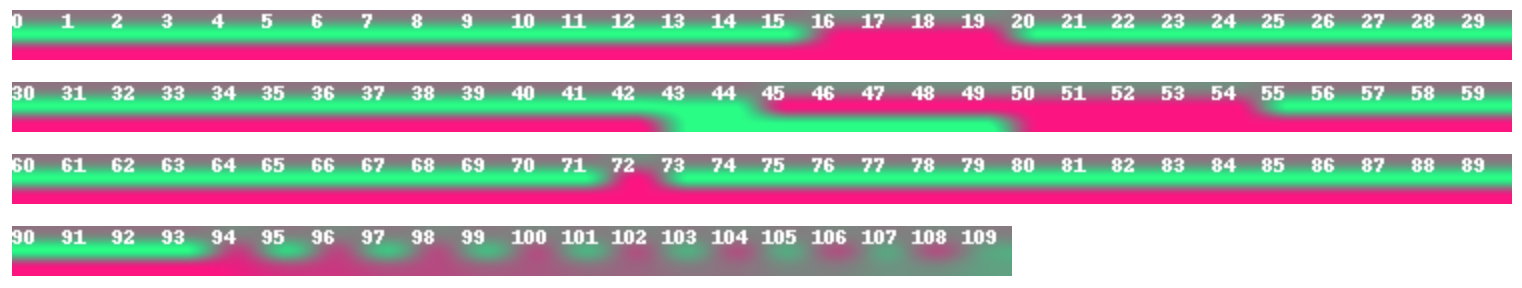
\includegraphics[width=\textwidth]{images/classifier/neuron-activations-simple-rnn-model-3/backflip-6-rasmus}\\
%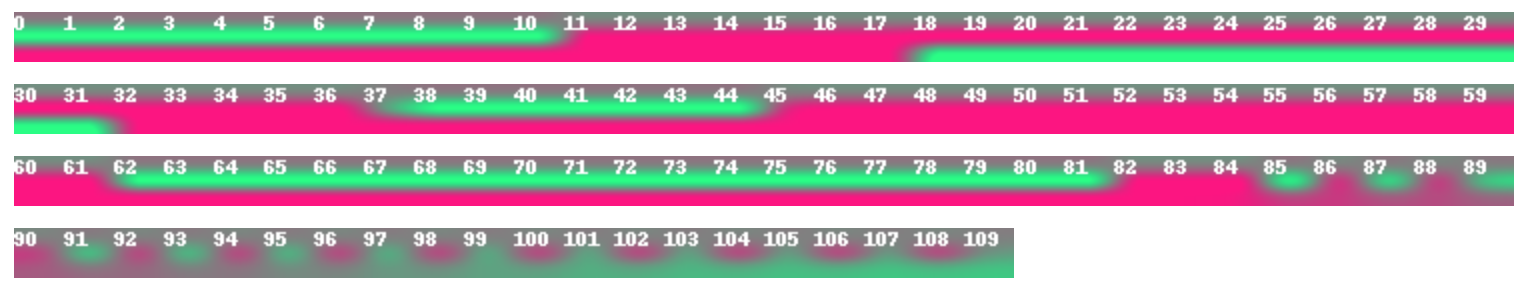
\includegraphics[width=\textwidth]{images/classifier/neuron-activations-simple-rnn-model-3/backflip-64-allar}\\
%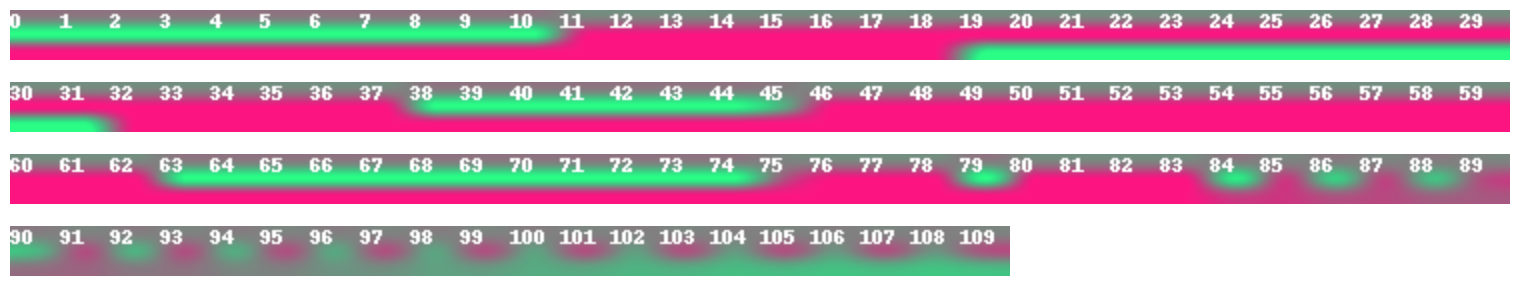
\includegraphics[width=\textwidth]{images/classifier/neuron-activations-simple-rnn-model-3/backflip-66-allar}\\
\end{tabular}
    \caption{Simple RNN neuron activations for backflip samples}
    \label{backflip-neuron-activations-simple-rnn}
\end{figure*}

\begin{figure*}
   \centering
\begin{tabular}{c}
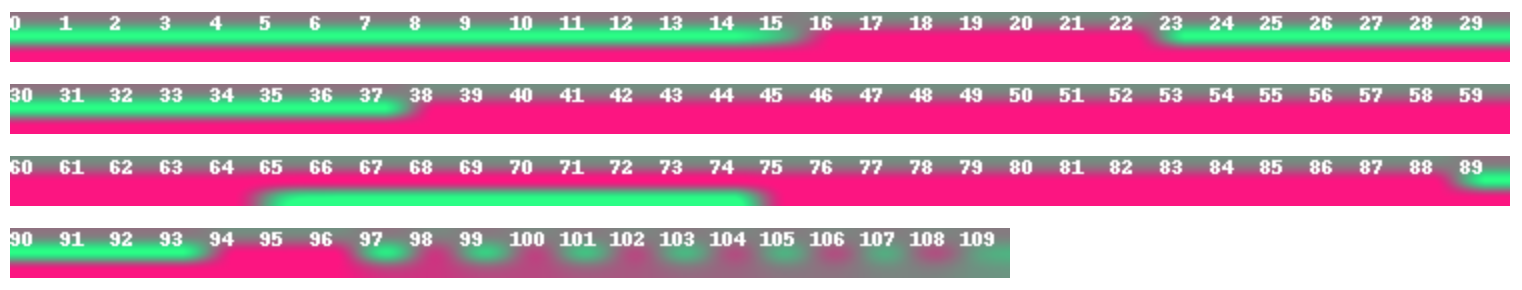
\includegraphics[width=\textwidth]{images/classifier/neuron-activations-simple-rnn-model-3/flack-19-rasmus}\\
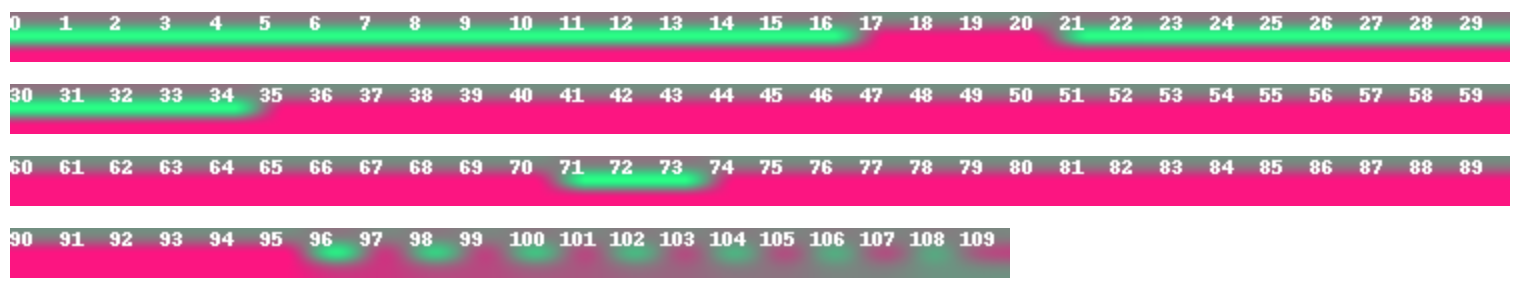
\includegraphics[width=\textwidth]{images/classifier/neuron-activations-simple-rnn-model-3/flack-31-rasmus}\\
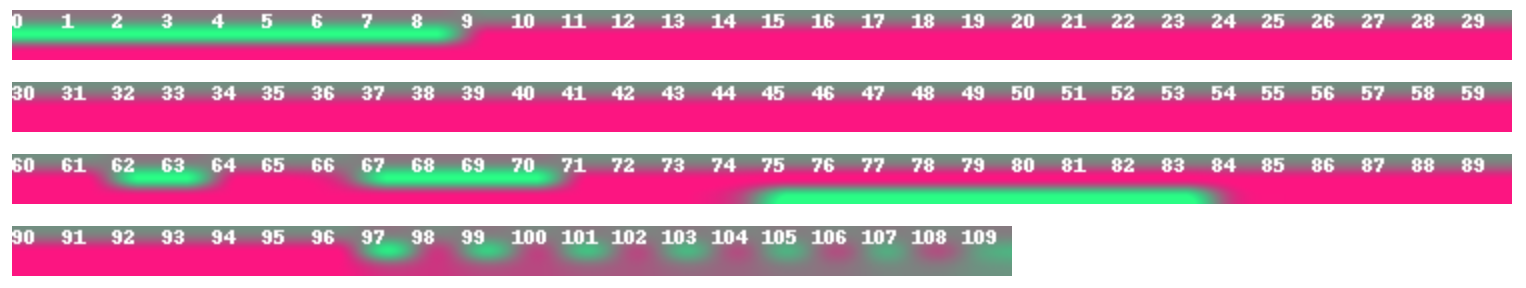
\includegraphics[width=\textwidth]{images/classifier/neuron-activations-simple-rnn-model-3/flack-55-martin}\\
%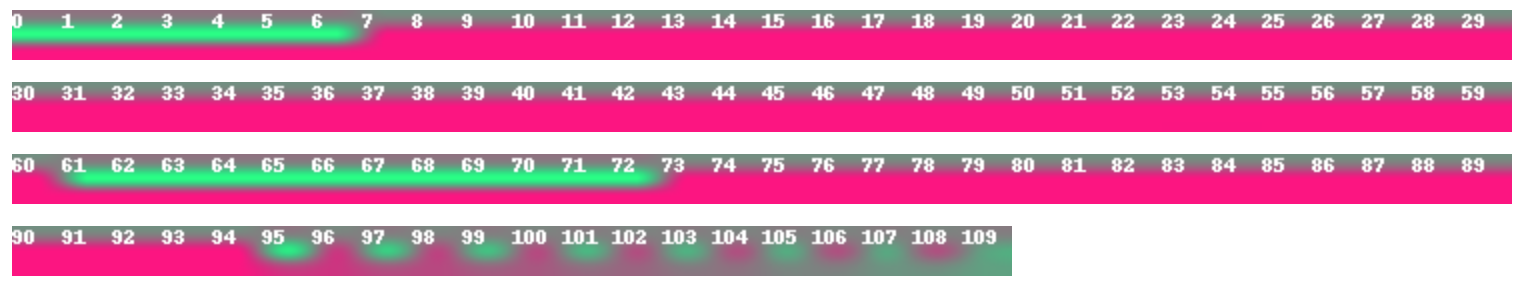
\includegraphics[width=\textwidth]{images/classifier/neuron-activations-simple-rnn-model-3/flack-59-martin}\\
%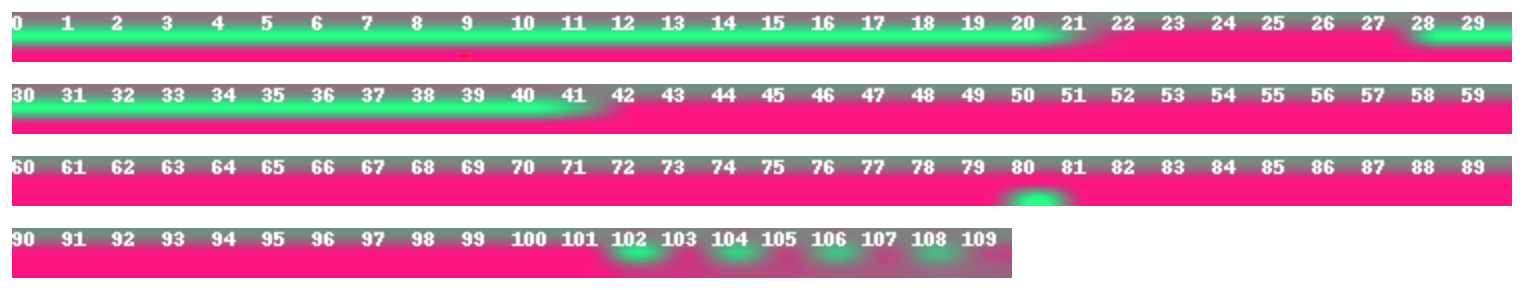
\includegraphics[width=\textwidth]{images/classifier/neuron-activations-simple-rnn-model-3/flack-68-rasmus}\\
\end{tabular}
    \caption{Simple RNN neuron activations for back handspring samples}
    \label{back-handspring-neuron-activations-simple-rnn}
\end{figure*}










